%---------------------------------------------------------------------------%
%->> Chapter 2: 相关技术与研究现状
%---------------------------------------------------------------------------%

\chapter{相关技术与研究现状}

微服务故障根因定位关注如何从复杂运行现象中识别真实故障源，是智能运维中的关键研究问题。随着大语言模型与智能体技术逐步进入智能运维领域，相关研究已不再仅关注异常检测结果本身，而是进一步延伸到诊断过程组织、工具交互协同以及历史经验复用等方面。为说明本文研究所依赖的技术基础与现有研究背景，本章将围绕微服务故障诊断和大语言模型智能体两方面内容展开，介绍相关基础概念，梳理传统方法与基于大语言模型的方法研究现状，并在此基础上总结现有工作的不足，为后续章节的方法设计提供背景支撑。

%---------------------------------------------------------------------------%
%->> 2.1 微服务故障诊断基础概念
%---------------------------------------------------------------------------%
%---------------------------------------------------------------------------%
%->> Section 2.1: 微服务故障诊断基础概念
%---------------------------------------------------------------------------%

\section{微服务故障诊断概述}

微服务架构将复杂业务拆分为多个可独立部署的服务单元，各服务围绕特定业务能力运行，并通过 HTTP 或 RPC 协同处理请求。这种组织方式提升了系统扩展性和迭代效率，也改变了故障的形成方式。故障不再局限于单一模块内部，还可能沿服务调用、资源竞争或基础设施依赖向外扩散，表现为跨服务、跨层级的异常。这种分布式特性使得故障的可观测性和可追溯性都面临新的挑战。

微服务故障诊断的难点主要来自三个方面。第一，业务逻辑被拆分到多个服务及其支撑组件中，根因容易隐藏在下游依赖内部，导致症状与根因在空间上出现分离。第二，系统通常运行在容器编排环境中，实例会随调度和负载持续变化，静态拓扑难以完整反映运行时依赖。第三，一次请求往往穿过网关、业务服务、缓存、消息队列和数据库等多个环节，任一环节异常都可能沿调用链向上传播，并在入口侧形成更明显的外部症状，从而掩盖真实根因的位置。

以电商系统为例，用户请求经由网关进入系统后，通常要经过订单、支付、库存等多个服务以及数据库、缓存等支撑组件。若支付数据库连接池耗尽，异常会先影响支付服务，再沿调用关系传递至订单服务和网关，最终表现为页面超时或请求失败。可见症状与真实根因之间往往隔着若干服务和依赖环节，这正是微服务场景与单体系统诊断的重要区别。这种传播链条的存在要求诊断方法必须具备回溯能力。

根因分析（Root Cause Analysis，RCA）的目标，是从外部异常现象出发，结合运行证据与逻辑推断识别导致故障的真实原因。与针对表面症状的临时处置不同，根因分析关注故障为何产生、异常如何传播，以及究竟哪个组件或关系构成根因。准确的根因定位能够为后续修复提供依据，并降低同类故障重复发生的概率，从而提升系统整体可靠性。

故障定位任务可形式化表述如下。设整个微服务系统由一组服务节点$S=\{S_1, S_2, \ldots, S_m\}$及其调用关系$E \subseteq S \times S$构成。每个服务节点$S_i$会持续产生多模态监控数据$D_i = \{T_i, M_i, L_i\}$，分别对应调用链路、指标和日志。在某一时刻$t$，系统触发异常检测模块，得到候选异常告警集合$A_t = \{a_1, a_2, \ldots, a_k\}$。根因定位函数可定义为$\theta: A_t \rightarrow S \cup E$。其中，$S_i$表示被判定为根因的故障服务节点，$e_{ij} = (S_i, S_j)$表示被判定为根因的故障调用链路。也就是说，给定异常告警集合$A_t$后，模型需要输出最可能导致系统整体异常的故障位置。

微服务环境下的根因分析还面临几类共性挑战。故障传播路径往往较长，相同症状背后可能对应不同根因，导致诊断存在多解性；系统运行状态持续变化，静态拓扑难以完整描述运行时依赖；可用于监督学习的故障实例相对稀缺，监督信号有限；指标、日志和调用链路之间又存在明显异构性。如何在保留各模态特征的同时建立稳定关联，是微服务故障诊断的核心问题。


%---------------------------------------------------------------------------%
%->> 2.2 大语言模型与智能体应用开发框架
%---------------------------------------------------------------------------%
%---------------------------------------------------------------------------%
%->> Section 2.2: 大语言模型与智能体应用开发框架
%---------------------------------------------------------------------------%

\section{大语言模型与智能体应用开发框架}

大语言模型（Large Language Model，LLM）是 Transformer 架构~\cite{vaswani2017attention}构建的深度学习模型。它通过大规模预训练获得通用语言表示，并在此基础上展现出对自然语言指令的理解能力。以 GPT 系列~\cite{openai2023gpt4}和 Qwen 系列~\cite{qwen2023technical}为代表的模型，在参数规模扩大后展现出较强的指令跟随、少样本学习和链式推理能力~\cite{wei2022chain}。因此，LLM 开始被用于承担复杂任务中的理解、规划与决策，逐步从语言生成工具转变为任务执行的核心推理引擎。

智能体（Agent）通常指能够感知环境、规划行动并执行操作以完成目标的系统~\cite{yao2022react}。在当前主流实现中，LLM 常作为核心推理引擎，负责理解任务意图、生成执行策略并协调任务流程。感知模块提供环境状态，执行模块负责具体操作，工具模块用于扩展外部信息获取和任务执行能力~\cite{hong2023metagpt}。相较于依赖显式规则的传统软件，这类系统更适合处理开放式任务，尤其是需要多步推进且中间状态难以预先枚举的任务。

从能力构成看，典型智能体系统通常包括记忆、规划、行动和工具使用四个部分~\cite{hong2023metagpt}。如图\ref{fig:agent-system-overview}所示，语言模型作为控制中心与这四类能力持续交互，还可进一步加入反思能力和多智能体协作~\cite{weng2023agent}。其中，记忆用于保存中间结果和历史状态，以支持跨步骤的上下文延续；规划负责分解任务并调整策略；行动负责执行 API 调用、数据库访问或代码操作。工具使用则让模型能够访问外部系统和实时信息，从而突破预训练知识的时效性限制。

\begin{figure}[htbp]
\centering
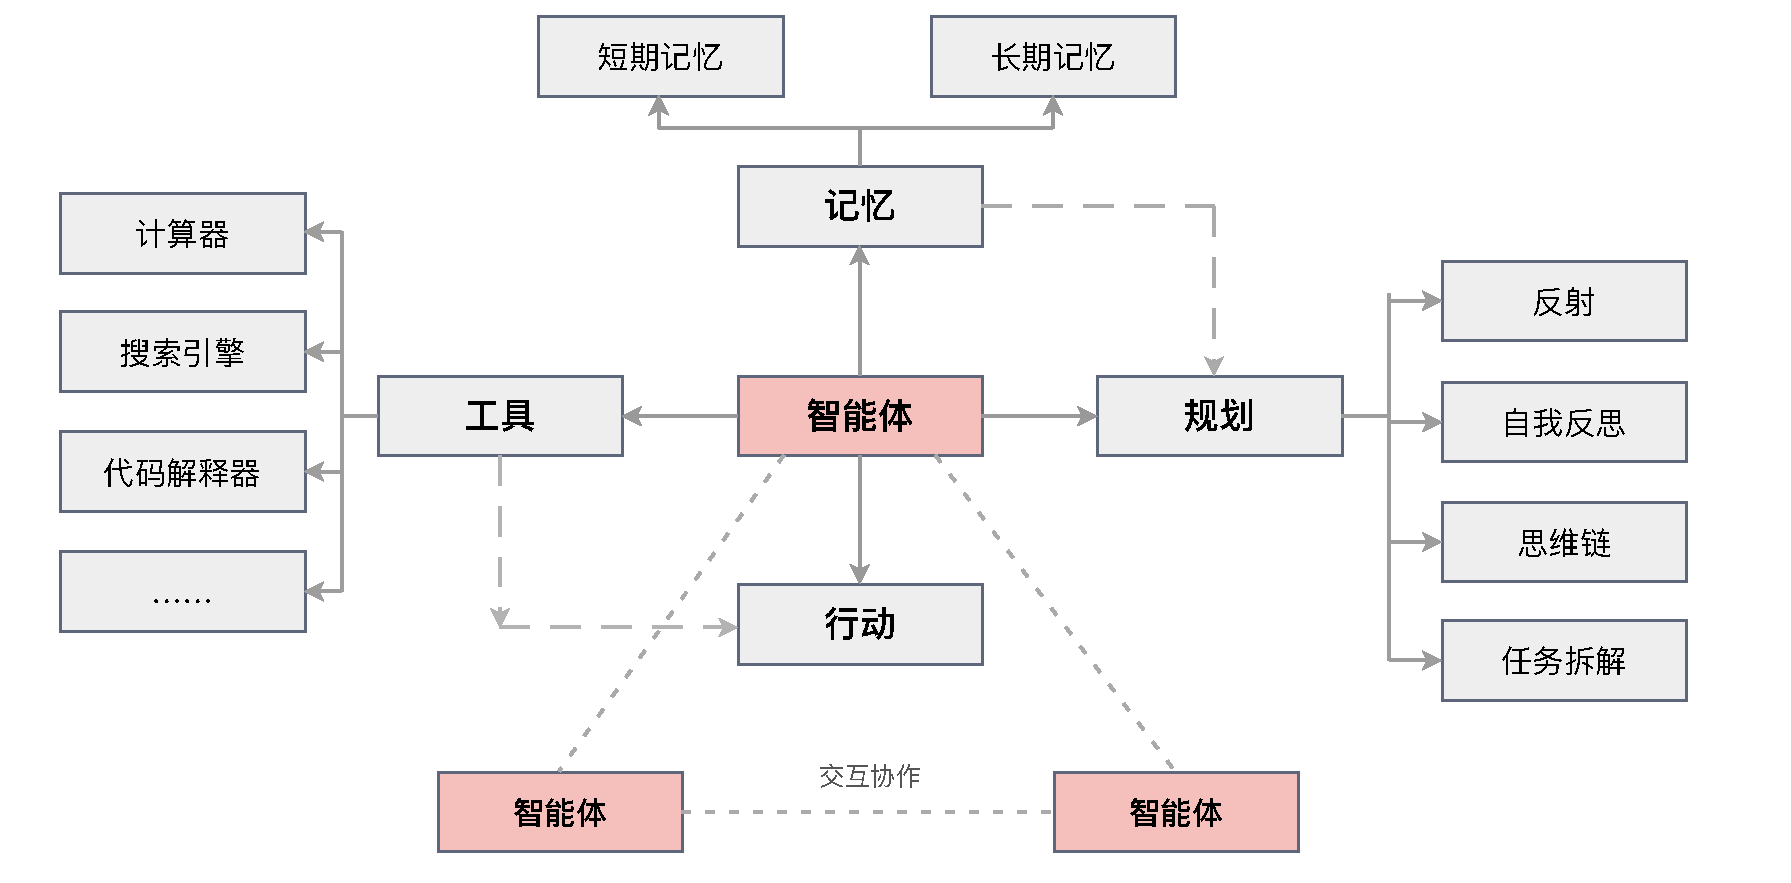
\includegraphics[width=0.95\textwidth]{Figures-Src/Chap2-RelatedWork/Agent/chart.pdf}
\bicaption{\enspace 智能体系统的典型组成（改绘自Weng~\cite{weng2023agent}）}{\enspace Typical Components of an Autonomous Agent System (Redrawn from Weng~\cite{weng2023agent})}
\label{fig:agent-system-overview}
\end{figure}

围绕智能体开发，业界已经形成两类常见支撑环境。一类是通用编排框架。LangChain 提供组件化构建方式，可将多个处理环节组织为链式结构~\cite{langchain}；LangGraph 在此基础上引入状态图机制，以支持更复杂的控制流和状态管理~\cite{langgraph}；Dify 则通过可视化界面配置工作流~\cite{dify}。这类框架更适合流程相对稳定、交互边界较清晰的任务，但在需要频繁调整执行路径的场景中灵活性受限。

另一类是面向真实执行场景的 AI 编程智能体环境。GitHub Copilot~\cite{copilot2024}和 Cursor~\cite{cursor2024}先后把代码补全、多文件问答和重构能力引入开发流程。进一步地，OpenAI Codex~\cite{codex2024}、OpenCode~\cite{opencode2025}、OpenClaw~\cite{openclaw2025}、Google Gemini CLI~\cite{gemini_cli2024}、阿里云 Qwen Code~\cite{qwen_code2025}和 Anthropic Claude Code~\cite{claudecode2024}将文件读写、命令执行和工具调用整合到统一环境中，使模型能够直接操作工程上下文，而不再局限于生成代码片段。



%---------------------------------------------------------------------------%
%->> 2.3 传统微服务故障诊断方法研究现状
%---------------------------------------------------------------------------%
%---------------------------------------------------------------------------%
%->> Section 2.3: 传统微服务故障诊断方法
%---------------------------------------------------------------------------%

\section{传统微服务故障诊断方法}

传统微服务故障根因定位方法大致可分为两类：因果推断的方法和特征学习的方法~\cite{microservice-diagnosis-survey}。前者试图显式恢复故障传播结构，并沿依赖关系回溯根因；后者从指标、日志和调用链路中提取判别性表示，直接完成异常定位、排序或分类。两类方法的主要区别在于知识来源不同：前者依赖显式结构，后者依赖数据驱动表示，这种差异决定了它们在不同场景下的适用性。

\subsection{因果推断方法}

这类方法的核心假设是，故障会沿服务调用、部署支撑和资源竞争等依赖关系逐步传播。因此，只要能够较准确地刻画传播结构并识别异常传播方向，就有可能沿传播路径回溯到根因组件~\cite{Pearl2009Causal,Spirtes2000Causation,pham2024causalmicroservicesurvey}。这一假设的有效性依赖于依赖关系的完整性和传播模式的稳定性。

\paragraph{因果图构建与结构发现}
一类工作先构建服务级或实例级依赖图，再结合因果发现或图排序方法恢复异常传播结构。CloudRanger~\cite{Wang2018Cloudranger}和MS-Rank~\cite{Ma2019Ms-rank}从服务依赖关系与监控指标出发构建图结构，并结合因果强度估计或多指标融合对异常传播进行排序。MicroDiag~\cite{Wu2021Microdiag}在组件依赖图基础上结合因果推断，完成更细粒度的性能诊断。ServiceRank~\cite{Ma2021Servicerank}则沿服务依赖图对候选根因进行排序，以提高大规模场景中的定位效率。此类方法共同强调依赖结构在故障传播中的作用，并借助显式图结构增强可解释性。

\paragraph{根因回溯与干预分析}
另一类工作在已有因果图或依赖图上执行根因回溯。MicroRCA~\cite{wu2020microrca}将节点异常程度和边关联强度编码为随机游走权重，并利用 PageRank 式排序~\cite{pagerank-page1999}生成根因候选；REASON~\cite{Wang2023Interdependent}面向相互依赖微服务场景构建跨层级因果网络，并结合带重启的随机游走执行根因定位。CIRCA~\cite{Li2022Causal}将根因定位建模为干预识别问题，通过因果贝叶斯网络中的条件分布变化识别潜在根因指标。近期综述还指出，不同因果发现和图推断方法在真实场景中的效果差异明显，而且对参数设定和数据质量较为敏感~\cite{pham2024causalmicroservicesurvey}。

这类方法的优势是结构清晰、结果可解释，但性能高度依赖图结构质量和因果关系恢复精度。若依赖关系不完整、系统拓扑持续演化，或监控数据存在噪声、稀疏性与概念漂移，沿图传播和干预推理都容易产生系统性偏差~\cite{pham2024causalmicroservicesurvey}。因此，因果推断方法在复杂动态场景下仍表现出较强的结构依赖，这限制了其在快速变化环境中的适用性。

\subsection{特征学习方法}

这类方法将故障诊断视为表征学习和模式识别问题，其核心是从指标、日志和调用链路中学习具有判别力的表示，并利用该表示完成异常检测、根因排序或故障分类。与因果方法相比，这类方法更强调从数据中自动提取特征，对复杂非线性关系具有更强的拟合能力，因而在数据充足时往往表现更好。

\paragraph{单模态特征学习方法}

早期研究多围绕单一模态构建故障表示。日志方向关注从运行日志中捕获异常模式。LogGPT~\cite{loggpt}利用 GPT 式生成模型建模日志序列，并通过强化学习微调策略提升异常检测性能；Landauer 等人~\cite{deep-learning-log-survey}系统梳理了循环神经网络、卷积神经网络和 Transformer 等架构在日志异常检测中的应用。指标方向主要从时序监控数据中检测异常并定位根因，代表工作包括 BARO~\cite{baro-rca}、RobustTAD~\cite{robusttad} 和 DCdetector~\cite{dcdetector}。链路方向则利用调用拓扑与时序关系进行故障定位。以 GAL-MAD~\cite{gal-mad}为例，该方法将微服务调用建模为时空图结构，并结合图注意力网络与长短期记忆网络学习依赖关系。

单模态方法各有优势，也各有明显边界。日志数据语义丰富，但噪声较多，解析质量依赖日志规范；指标数据便于发现数值异常，但难以直接解释故障原因；链路数据能描述传播路径，却难以捕获资源竞争和语义线索。随着这些限制逐渐显现，研究重心开始转向多模态融合。

\paragraph{多模态特征学习方法}

多模态方法同时利用指标中的数值异常、日志中的语义线索和链路中的依赖关系，以形成更完整的故障表示。现有工作大致沿三条路线展开：一是图神经网络的方法，将微服务系统建模为服务依赖图并学习节点表示；二是对比学习方法，通过共享表示提取跨模态不变特征；三是将因果建模与深度学习结合，在表示学习中显式考虑传播关系。

DiagFusion~\cite{zhang2023robust}验证了指标、日志和链路三种模态融合在微服务故障诊断中的有效性；AnoFusion~\cite{anofusion}利用图变换网络建模异构多模态数据间的关联；CHASE~\cite{chase-zhao2024}在多模态图表示学习框架中引入因果超图，以刻画异常在调用路径上的传播关系。TVDiag~\cite{tvdiag}通过统一不同模态的故障视图提高跨场景泛化能力；DynaCausal~\cite{dynacausal}则进一步考虑时序演化和动态依赖。相较于单模态方法，这类方法通常能更充分地利用不同观测信号之间的互补关系。

但多模态特征学习方法仍有局限。其表示往往与特定任务、数据集和故障分布紧密绑定；监督式方法依赖标注样本，无监督方法虽然降低了标注负担，却更偏向异常分离而非经验复用；图神经网络和深度时序模型的内部决策过程不够透明，跨系统迁移时容易受到拓扑差异和模态分布变化的影响~\cite{zhang2023robust,sun2024art}。这种对特定数据分布的依赖限制了方法的泛化能力。

总体来看，传统方法虽然在固定基准和已知故障场景下取得了较好效果，但知识形态仍偏静态。因果推断方法依赖预先构建或离线学习的图结构，特征学习方法依赖围绕特定任务训练出的表示模型。当系统拓扑持续变化或新型故障不断出现时，这些方法往往需要重新建图、重新训练，或反复调整参数。更重要的是，现有表示大多服务于单次定位，难以直接支持相似故障检索与诊断知识绑定，缺乏从历史经验中持续积累的机制。传统方法因此仍缺少一种可独立于具体下游模型的统一故障表征。第三章提出的故障指纹方法正是针对这一缺口展开。


%---------------------------------------------------------------------------%
%->> 2.4 大语言模型驱动的根因定位方法
%---------------------------------------------------------------------------%
%---------------------------------------------------------------------------%
%->> Section 2.4: 大语言模型驱动的根因定位方法
%---------------------------------------------------------------------------%

\section{大语言模型驱动的根因定位方法}

传统方法在已知故障场景下取得了一定效果，但在动态环境中仍难以统一组织多源证据，也缺乏交互式诊断和历史经验的灵活复用。为缓解这些问题，研究者开始将大语言模型引入微服务故障根因定位任务，以期利用其语言理解和推理能力弥合不同模态之间的语义鸿沟。现有工作大致可分为四类：大语言模型离线分析、工具增强的单智能体、多智能体协同诊断，以及知识增强的多智能体协同诊断。

\subsection{大语言模型离线分析}

早期方法将大语言模型放在诊断流程末端。系统先完成告警聚合、诊断信息收集和上下文组织，再把整理后的材料交由大语言模型生成根因报告、故障摘要或处置建议。在这类方法中，大语言模型主要负责理解和组织已有证据，而不直接参与在线诊断过程。

Ahmed 等人\cite{ahmed2023recommending}较早系统评估了大语言模型在云故障根因与缓解建议生成中的可行性； GPT-4 上下文学习的自动根因分析方法\cite{zhang2024gpt4iclrca}表明，不依赖持续微调也能生成较高质量的根因建议。PACE-LM\cite{zhang2023pacelm}在推荐阶段加入置信度估计，以降低幻觉输出误导值班工程师的风险。X-lifecycle Learning\cite{goel2024xlifecycle}尝试将代码、配置和监控等信息统一纳入上下文；eARCO\cite{goel2025earco}进一步利用提示优化和相似案例增强改进推荐质量。这些工作说明，即使只在流程末端使用模型，大语言模型也能改善事件摘要、案例对齐和根因解释。

在系统实现层面，RCACopilot\cite{chen2024rcacopilot}将告警、运行时诊断信息与历史事件组织为统一输入，再由模型生成根因类别和解释性叙述；Xpert\cite{xpert-jiang2024}根据故障上下文推荐诊断查询，以减少人工编写运维 DSL 的工作量。Cloud Atlas\cite{xie2024cloud}利用大语言模型结合系统文档、遥测和部署信息自动构建因果图，并通过额外验证步骤提高可靠性。但这类方法处理的仍然是预先整理好的材料。一旦证据不足，模型既无法主动发起新的观测请求，也难以根据中途结果调整排查方向。后续工作因此转向让模型直接调用外部工具。

\subsection{工具增强的单智能体}

工具增强的单智能体方法将大语言模型引入诊断过程。与离线分析不同，这类方法不再只处理事先整理好的材料，而是让模型通过工具调用访问日志、指标、数据库或拓扑信息，并根据观察结果决定下一步动作。诊断过程因此由离线总结转向在线交互，模型从被动接收者转变为主动探索者。

在通用方法层面，ReAct\cite{yao2022react}为语言模型结合推理与行动提供了统一范式，ToolFormer 和 ToolLLM\cite{schick2024toolformer,qin2023toolllm}增强了模型调用外部工具和真实 API 的能力。在根因定位场景中，Roy 等人\cite{roy2024exploringllmrca}系统评估了配备检索与诊断服务接口的 ReAct 智能体，指出主动收集日志、指标和数据库信息能够缓解离线分析中的信息不足问题。RCAgent\cite{wang2024rcagent}在工业云环境中加入上下文管理、自一致动作序列和输出稳定化机制，使单智能体更接近真实可用。

后续工作主要围绕如何提高单智能体诊断稳定性来展开。K8sGPT\cite{k8sgpt2023}是较早的大语言模型辅助 Kubernetes 排障工具，它通过 analyzers 检查集群对象，并结合事件和资源状态生成诊断说明；SynergyRCA\cite{xiang2025synergyrca}用 StateGraph 和 MetaGraph 提供更结构化的 RCA 上下文。MicroRCA-Agent\cite{tang2025microrcaagent}将日志压缩、链路异常筛选和跨模态提示融合到统一流程中；GALA\cite{tian2025gala}则将结构化传播线索与语言推理结合起来。与离线分析相比，这类方法已经能够在诊断过程中持续观察、推理，并根据中途结果调整动作。

然而，这种方式的负担也逐渐集中到单个智能体内部。随着可调用工具和上下文范围不断扩大，日志检索、证据解释、工具选择、路径调整和结论生成等职责都压在同一个执行体上。动作链变长或上下文堆积时，系统稳定性就会明显下降\cite{roy2024exploringllmrca,wang2024rcagent,xiang2025synergyrca,tang2025microrcaagent}。这种单点负载过重的问题促使后续研究开始将不同职责拆分给多个角色。

\subsection{多智能体协同诊断}

多智能体协同诊断方法进一步把诊断过程拆分给多个角色。与工具增强的单智能体不同，这类方法不再由单个智能体承担日志检索、证据解释、路径选择和结论生成等全部职责，而是将告警理解、数据检索、依赖分析、根因判断和处置建议分配给不同角色，并利用角色之间的交叉验证降低单点推理失误带来的影响。

在通用研究中，MetaGPT\cite{hong2023metagpt}和 Multi-LLM Agent\cite{small-llm-agents}都表明，将复杂任务拆分为不同角色，通常比让单个模型承担全部职责更稳定。放到 RCA 场景中，mABC（Multi-Agent Blockchain-inspired Collaboration，多智能体区块链协同）\cite{zhang2024mabc}通过七类专用智能体组成协作流水线，并引入区块链式投票机制缓解单点幻觉；Nissist\cite{an2024nissist}围绕 TSG 理解、检索和计划生成构建多智能体故障处置辅助系统。相较于单智能体，这类方法的关键变化在于把错误风险分散到多个决策环节。

进一步的工作开始转向协作过程本身的控制。 Monte Carlo Tree Search 的多智能体故障定位系统\cite{ren2025mctsfaultlocalization}尝试用树搜索和知识奖励机制控制服务级探索顺序；RCLAgent\cite{zhang2025rclagent}借鉴人工 RCA 中递归展开和跨模态推理的特点，提出 multi-agent recursion-of-thought 框架。相应地，多智能体方法关注的已不只是角色分工，还包括协作方式和停止条件。

不过，多智能体并未从根本上消除诊断不稳定问题。角色数量增加后，消息传递、共享状态维护、协作顺序和停止条件都会成为新的系统负担。若机制设计不当，系统容易退化为冗长交互、重复取证，甚至出现不同角色相互冲突的判断，反而降低诊断效率。后续研究因此开始进一步引入 SOP、TSG、规则库和显式工作流，以减少开放式协作带来的不确定性。

\subsection{知识增强的多智能体协同诊断}

知识增强的多智能体协同诊断方法进一步把已有知识纳入诊断过程。与前一类方法相比，这类工作不再主要依赖角色之间的开放式协作，而是将排障指南、标准操作规程（Standard Operating Procedure，SOP）、故障排查指南（Troubleshooting Guide，TSG）和历史案例转化为执行约束，通过离线编译、在线检索或动作限制等方式缩小动作空间，从而提高诊断的稳定性和可预测性。

这类方法在知识使用方式上存在差异。LLexus\cite{lascasas2024llexus}将自然语言 TSG 转化为可执行计划，再让智能体按计划执行；Nissist\cite{an2024nissist}从 TSG 和历史缓解记录中抽取知识并构建知识库；Flow-of-Action\cite{pei2025flowofaction}通过 Thought-ActionSet-Action 范式，将 SOP 约束嵌入多智能体动作选择过程。共同点在于，已有经验不再只是参考材料，而被转化为角色需要遵守的执行约束。

\begin{figure}[tbp]
\centering
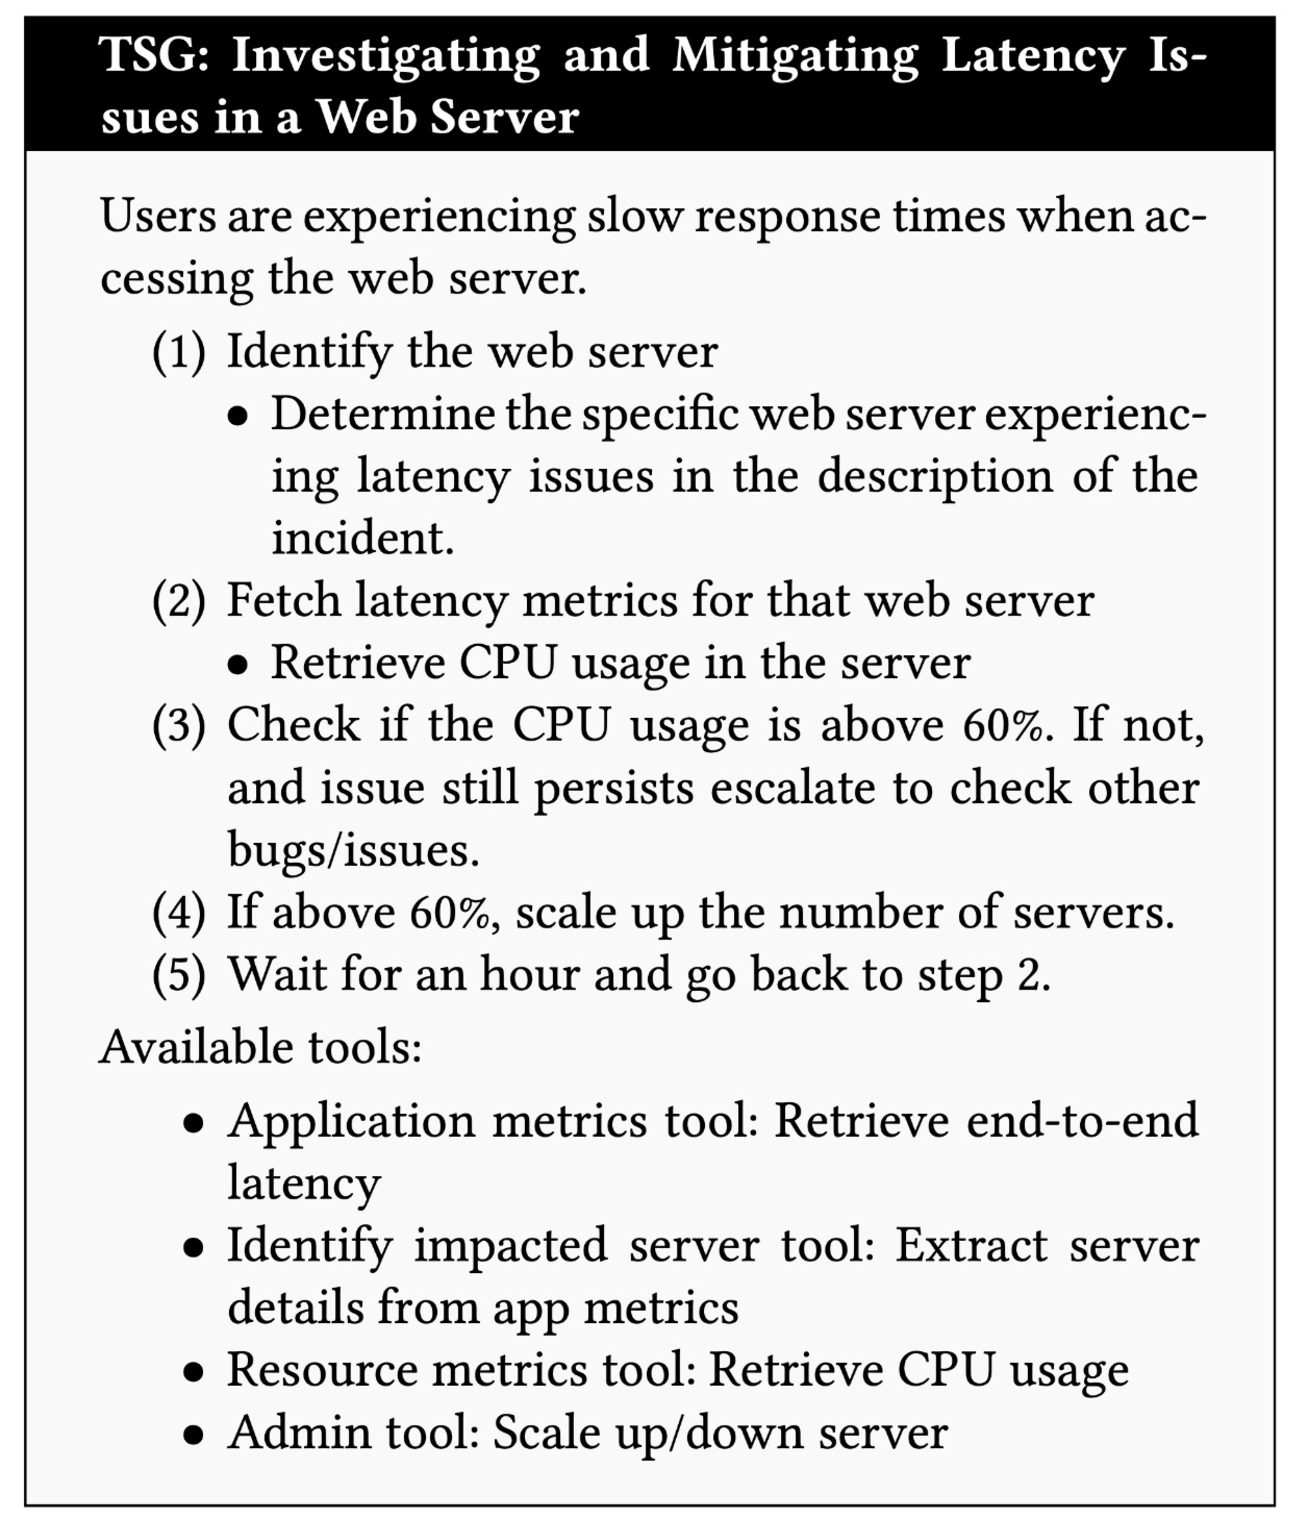
\includegraphics[width=0.54\textwidth]{Figures-Src/Chap2-RelatedWork/tsg/chart.pdf}
\bicaption{\enspace LLexus 中的 TSG 片段示例\cite{lascasas2024llexus}}{\enspace TSG Snippet from LLexus\cite{lascasas2024llexus}}
\label{fig:llexus_tsg_example}
\end{figure}

图\ref{fig:llexus_tsg_example}给出了 LLexus\cite{lascasas2024llexus} 中的一段 TSG。图中直接写出了问题描述、排查步骤和可调用工具，也说明这类方法对既有 TSG 的质量和覆盖范围依赖较强。

另一组工作更进一步，将知识直接编译为工作流。ARCAS\cite{demarne2024arcas}通过 DSL 化的 Auto-TSG 库组织并行诊断逻辑，再由 LLM 对多路输出进行优先级判断；StepFly\cite{mao2025agentictsgautomation}将 TSG 质量改进、执行 DAG 抽取和在线 scheduler-executor 执行整合在一起。FastReject\cite{fastreject2025}则体现出“在线诊断 + 离线规则演进”的思路。发展到这一步，知识已不再只是辅助材料，而成为诊断流程的一部分。

但这类方法仍未彻底解决问题。知识增强确实提升了稳定性，但许多系统仍依赖人工整理或离线整理好的 SOP、TSG 和规则库，因此知识获取与更新成本较高\cite{an2024nissist,lascasas2024llexus,mao2025agentictsgautomation}。近期针对 RCA 智能体的过程级失败分析也表明，即便加入知识约束，数据解释错误、探索不完整和角色通信失效等问题仍然存在\cite{kim2026agentfailurerca}。总体上，现有工作大多仍停留在调用既有 SOP、TSG 和规则库，而缺乏从真实诊断过程中自动提取和演化知识的能力。稳定的故障表征、从真实诊断过程自动生成 SOP 的方法，以及把 SOP 在线执行、必要探索和后续更新串联起来的机制，仍然是有待解决的三个基础问题。第三章正是围绕这三点展开。


%---------------------------------------------------------------------------%
%->> 2.5 本章小结
%---------------------------------------------------------------------------%
%---------------------------------------------------------------------------%
%->> Section 2.5: 本章小结
%---------------------------------------------------------------------------%

\section{本章小结}

本章回顾了微服务故障诊断的基础概念，并梳理了传统方法与大语言模型的方法。表\ref{tab:methods-comparison}比较了各类方法的主要做法和局限。

\begin{table}[H]
\centering
\bicaption{\enspace 微服务故障诊断方法及其局限}{\enspace Microservice Fault Diagnosis Methods and Their Limitations}
\label{tab:methods-comparison}
\renewcommand{\arraystretch}{1.3}
\small
\setlength{\tabcolsep}{5pt}
\begin{tabularx}{\textwidth}{>{\centering\arraybackslash}p{2.3cm}>{\centering\arraybackslash}p{2.1cm}>{\raggedright\arraybackslash}X>{\raggedright\arraybackslash}X}
\toprule
\rowcolor{lightgray!30}
\textbf{类别} & \textbf{子类别} & \textbf{主要做法} & \textbf{主要局限} \\
\midrule
\textbf{传统方法} & 因果推断 & 根据依赖图或因果图追踪异常传播并回溯根因 & 依赖图质量与先验假设，动态适应能力有限 \\
\cline{2-4}
& 特征学习 & 从指标、日志和调用链路中学习表示，用于定位或排序 & 依赖训练数据，泛化与可解释性受限 \\
\midrule
\textbf{大语言模型的方法} & 大语言模型离线分析 & 把整理后的告警、日志或工单交给大语言模型生成解释与建议 & 依赖预先整理输入，缺乏在线补证能力 \\
\cline{2-4}
& 工具增强的单智能体 & 通过工具调用主动收集证据并在线推理 & 长链路交互下稳定性与效率受限 \\
\cline{2-4}
& 多智能体协同诊断 & 将检索、分析和结论生成分给不同角色协作完成 & 协作开销较高，流程控制困难 \\
\cline{2-4}
& 知识增强的多智能体协同诊断 & 将 SOP、TSG 或规则库纳入诊断流程，限制推理与执行范围 & 知识获取与更新成本高，对覆盖范围依赖较强 \\
\bottomrule
\end{tabularx}
\setlength{\tabcolsep}{6pt}

\end{table}

表\ref{tab:related-work-comparison}进一步从知识来源、知识形式、在线诊断、知识更新和 SOP 未覆盖时的处理五个方面，对 LLexus、Flow-of-Action、FastReject 和本文进行比较。

\begin{table}[H]
\centering
\bicaption{\enspace 本文工作与 LLexus、Flow-of-Action 和 FastReject 的对比}{\enspace Comparison Between This Work, LLexus, Flow-of-Action, and FastReject}
\label{tab:related-work-comparison}
\renewcommand{\arraystretch}{1.3}
\footnotesize
\setlength{\tabcolsep}{4pt}
\begin{tabularx}{\textwidth}{>{\raggedright\arraybackslash}p{2.2cm}>{\raggedright\arraybackslash}X>{\raggedright\arraybackslash}X>{\raggedright\arraybackslash}X>{\raggedright\arraybackslash}X}
\toprule
\rowcolor{lightgray!30}
\textbf{比较项} & \textbf{LLexus} & \textbf{Flow-of-Action} & \textbf{FastReject} & \textbf{本文工作} \\
\midrule
知识来源 & 人工编写的 TSG & 既有 SOP 文档 & 人工定位结果与经验规则 & \textbf{故障注入生成的 SOP执行轨迹与复核后的在线案例} \\
知识表示 & 可执行计划 & SOP 流程 & 规则库与 SOP 校验路径 & \textbf{可执行 SOP（与故障指纹绑定）} \\
知识更新 & 人工维护 & 未强调持续更新 & 根据人工真值更新规则库 & \textbf{自动构建并增量更新} \\
在线诊断 & 按计划执行 & 在 SOP 约束下由多智能体执行 & 推理结果再经规则与 SOP 复核 & \textbf{由 SOP 驱动在线诊断} \\
诊断规程遵照 & 依赖既有 TSG & 主要受 SOP 覆盖范围限制 & 规则外推能力有限 & \textbf{逃逸机制支持继续排查} \\
\bottomrule
\end{tabularx}
\setlength{\tabcolsep}{6pt}
\end{table}

传统方法主要沿因果推断和特征学习两条路线展开。前者依赖显式传播结构，后者依赖从多模态观测中学习的判别表示，但两类方法都较少把历史经验沉淀为可直接复用的诊断流程，导致知识难以在不同故障场景间迁移。

大语言模型的方法则经历了从离线分析到在线交互、再到知识约束的演进。大语言模型离线分析提升了对既有材料的归纳能力，但在证据不足时缺乏主动补证能力；工具增强的单智能体开始通过工具调用直接获取日志、指标和链路信息，但在长链路任务中容易出现上下文过载。多智能体协同诊断通过角色分工缓解单体压力，却带来更高的协作与控制成本。知识增强的方法将 SOP、TSG 和规则库纳入执行过程，稳定性有所改善，但知识获取与更新仍然依赖人工，难以适应快速变化的故障模式。

综合来看，现有研究虽然已经覆盖故障分析、工具调用和知识约束，但仍较少把故障表征、SOP 构建和在线诊断组织成一套能够持续更新的方法，缺乏从诊断过程中自动提取和演化知识的机制。这正是第三章要解决的问题。

